\section{问题一：有界测角误差下的定位区域}
\subsection{半平面交模型}
令 $u(\theta)=(\cos\theta,\sin\theta)$，二维叉积记为 $\operatorname{cross}(a,b)=a_xb_y-a_yb_x$。第 $i$ 次观测的可行楔形写成
\begin{equation}\label{eq:wedge}
W_i=\{g:\operatorname{cross}(u(\theta_i-\varepsilon),g-p_i)\ge0,\quad \operatorname{cross}(u(\theta_i+\varepsilon),g-p_i)\le0\}.
\end{equation}
将式 \eqref{eq:wedge} 改写为 $A_i g\le b_i$，即可用线性规划检查空集和无界性；有界时枚举约束直线交点，再取凸包得到 $\mathcal P=\cap_iW_i$。与人为设置一个大正方形相比，该做法能明确返回 EMPTY、UNBOUNDED 或 BOUNDED 三种状态。

考虑接收区域时，程序将半径 $R$ 的圆盘替换为外切正 $K$ 边形，默认 $K=128$。其最大径向膨胀为 $R(\sec(\pi/K)-1)$，所以所得区域是安全外包，不把外包直径误写成曲边区域的精确直径。

\subsection{直径与最小包围圆}
对凸多边形顶点按逆时针排列，直径由一对对踵点取得，使用旋转卡壳计算；同时用顶点对穷举作独立数值对照。最小包围圆采用随机增量算法，再遍历全部顶点复核包含性，这两个几何子程序分别对应旋转卡壳和最小包围圆的经典做法\cite{toussaint,welzl}。只有
\begin{equation}\label{eq:clear-cert}
R^*(\mathcal P_{\rm out})\le 19.75\,\mathrm m
\end{equation}
时才向圆心发出清除请求，$0.25\,\mathrm m$ 用于数值余量。

\subsection{求解步骤与数值核验}
实现先将所有楔形边界和接收圆盘外切多边形统一写成半平面约束，再枚举约束直线交点。落在全部半平面内的交点按极角排序形成凸多边形；若交点不足以形成有界区域，则分别返回空集或无界状态，不进入清除流程。对有界多边形，旋转卡壳给出直径，随机增量算法给出最小包围圆，并用“所有顶点到圆心的距离不超过半径”作最后复核。该流程把数值几何、清除判定和协议动作分开，便于定位误差来源。

\begin{table}[H]\centering\small
\caption{问题一构造数据的逐步收缩核验}\label{tab:q1-shrink}
\begin{tabular}{rrrr}
\toprule
累计检测点数 & 外包面积 ($\mathrm m^2$) & MEC 半径 ($\mathrm m$) & 清除判定 \\
\midrule
1 & 39279.93 & 750.23 & 否 \\
2 & 2092.03 & 42.56 & 否 \\
3 & 658.61 & 22.52 & 否 \\
\bottomrule
\end{tabular}
\source{results/synthetic/q1.json；由相同构造数据逐次加入观测得到。}
\end{table}

表 \ref{tab:q1-shrink} 中第三次观测已经把区域直径压到 $39.00\,\mathrm m$，但最小包围圆半径仍为 $22.52\,\mathrm m$，因此按照式 \eqref{eq:clear-cert} 不应直接清除。对偶指标的同时记录避免了将“区域面积变小”误作“满足光学距离证书”；完整收缩过程见图~\ref{fig:q1-shrink}。

\begin{figure}[H]\centering
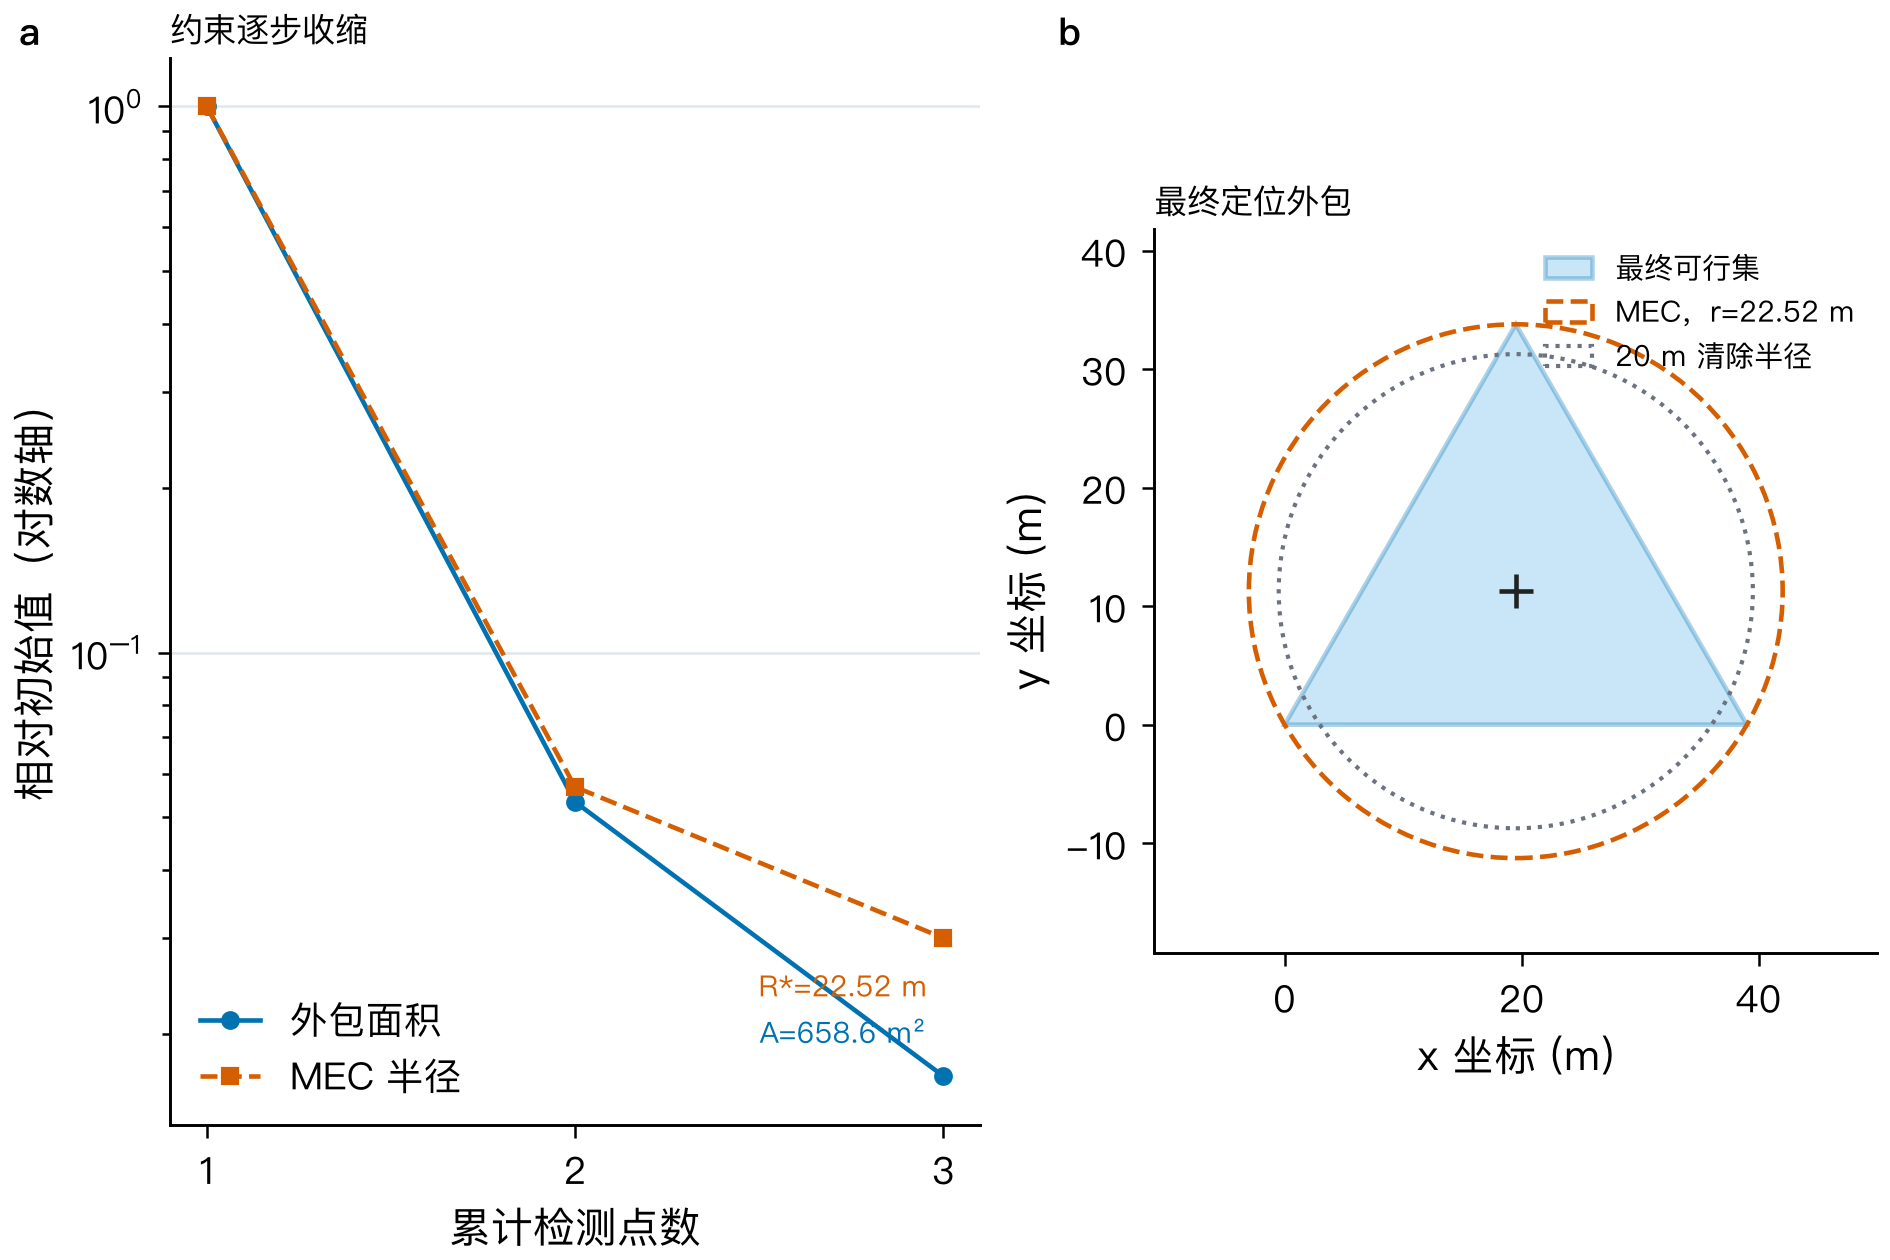
\includegraphics[width=0.98\linewidth]{figures/process_q1_intersection.png}
\caption{测向约束收缩过程与最终清除阈值核对}\label{fig:q1-shrink}
\source{results/synthetic/q1.json；左图为归一化收缩曲线，右图为最终可能区域与包围圆。}
\end{figure}

\subsection{“直径不超过40米”不是充分条件}
构造边长 $39\,\mathrm m$ 的等边三角形。其直径为 $39\,\mathrm m$，而最小包围圆半径为
\begin{equation}
R^*=\frac{39}{\sqrt3}=22.5167\,\mathrm m>20\,\mathrm m.
\end{equation}
因此直径上限不能替代最小包围圆判据。该反例也说明，清除判定必须针对整体可能区域，而不是将多次测向的交会点取平均。

图~\ref{fig:q1-counter} 用同一反例显示两种判据的差别；图~\ref{fig:q1-mec} 则给出多次楔形交集与最小包围圆的几何示意。

\begin{figure}[H]\centering
\begin{tikzpicture}[scale=0.08]
\coordinate (A) at (0,0);\coordinate (B) at (39,0);\coordinate (C) at (19.5,33.775);
\draw[thick] (A)--(B)--(C)--cycle;\draw[dashed] (19.5,11.258) circle (22.517);
\fill (19.5,11.258) circle (1.1);\draw[<->] (A)--(B) node[midway,below] {$39\,\mathrm m$};
\node at (19.5,-9) {直径 $39$ 米，但包围圆半径 $22.52$ 米};
\end{tikzpicture}
\caption{问题一的等边三角形反例}\label{fig:q1-counter}
\source{构造数据，数值来自 results/synthetic/q1.json。}
\end{figure}

\begin{figure}[H]\centering
\begin{tikzpicture}[x=1cm,y=1cm]
\draw[gray!60] (-3,-2.2) rectangle (3.2,2.4);\draw[thick] (-2.5,-1.5)--(2.4,-1.5)--(1.0,1.8)--cycle;
\draw[dashed] (0.0,0.1) circle (1.35);\fill (0,0.1) circle (1.5pt);
\node at (0,-2.7) {楔形交集 $\mathcal P$ 与最小包围圆};
\end{tikzpicture}
\caption{多次测向逐步收缩可能区域的示意}\label{fig:q1-mec}
\source{几何示意图；实际算法使用外切圆盘和凸多边形顶点。}
\end{figure}
